\documentclass{exam-zh}
\usepackage{siunitx}

\examsetup{
	page/size=a4paper,
	paren/show-paren=true,
	paren/show-answer=true,
	fillin/show-answer=true,
	solution/show-solution=true
}

\ExamPrintAnswerSet{
	sealline/show=true,
	page/size=a3paper,
	paren/show-answer=false,
	fillin/show-answer=false,
	solution/show-solution=false,
}


\everymath{\displaystyle}

\title{}
\subject{深度学习参考习题()}

\begin{document}

\maketitle


\begin{question}[points = 2]
	什么情况下神经网络模型被称为深度学习模型? \paren[A]

	\begin{choices}
		\item 加入更多层,使神经网络的深度增加
		\item 有维度更高的数据
		\item 当这是一个图形识别的问题时
		\item 以上都不正确
	\end{choices}
\end{question}

\begin{question}
	下面哪项操作能实现跟神经网络中 Dropout 的类似效果? \paren[B]
	\begin{choices}
		\item Boosting
		\item Bagging
		\item Stacking
		\item Mapping
	\end{choices}
\end{question}

\begin{question}
	下列哪一项在神经网络中引入了非线性? \paren[B]
	\begin{choices}
		\item 随机梯度下降 
		\item 修正线性单元 (ReLU) 
		\item 卷积函数 
		\item 以上都不正确
	\end{choices}
\end{question}

\begin{question}
	深度学习是当前很热门的机器学习算法,在深度学习中,涉及到大量的矩阵相乘,现在需要计算三个稠密矩阵 $A, B, C$ 的乘积 $ABC$,假设三个矩阵的尺寸分别为 $m \times n$,$n \times p$, $p \times q$,且 $m < n < p < q$,以下计算顺序效率最高的是\paren[A]
	\begin{choices}
		\item $(AB)C$
		\item $AC(B)$
		\item $A(BC)$
		\item 所有效率相同
	\end{choices}
\end{question}

\begin{question}
	输入图片大小为200 $\times$ 200,依次经过一层卷积(kernel size 5 $\times$ 5, padding 1, stride 2), pooling (kernel size 3$\times$3, padding 0, stride 1),又一层卷积(kernel size 3$\times$3, padding 1, stride 1)之后,输出特征图大小为 \paren[C]
  	\begin{choices}
		\item 95
		\item 96
		\item 97
		\item 98
	\end{choices}
	\begin{solution}
		输出大小为 $\left \lfloor (n - k + 2p + s) / s \right \rfloor $,故 $\left \lfloor (200 - 5 + 2 \times 1 + 2) / 2 \right \rfloor = 99$,
		
		$\left \lfloor (99 - 3 + 2 \times 0 + 1) / 1 \right \rfloor = 97$,$\left \lfloor (97 - 3 + 2 \times 1 + 1) / 1 \right \rfloor = 97$
	\end{solution}
\end{question}

\begin{question}
	神经网络模型(Neural Network) 因受人类大脑的启发而得名,神经网络由许多神经元(Neuron)组成, 每个神经元接受一个输入,对输入进行处理后给出一个输出,如下图所示。请问下列关于神经元的描述中,哪一项是正确的? \paren[E]
	\begin{choices}
		\item 每个神经元可以有一个输入和一个输出
		\item 每个神经元可以有多个输入和一个输出
		\item 每个神经元可以有一个输入和多个输出
		\item 每个神经元可以有多个输入和多个输出
		\item 上述都正确
	\end{choices}
\end{question}


\begin{question}
	如果我们用了一个过大的学习速率会发生什么? \paren[D]
	\begin{choices}
		\item 神经网络会收敛 
		\item 不好说 
		\item 都不对 
		\item 神经网络不会收敛
	\end{choices}
\end{question}

\begin{question}
	在一个神经网络中,下面哪种方法可以用来处理过拟合? \paren[D]
	\begin{choices}
		\item Dropout
		\item 分批归一化(Batch Normalization)
		\item 正则化(regularization)
		\item 都可以
	\end{choices}
\end{question}

\begin{question}
	批规范化(Batch Normalization)的好处 \paren[A]
	\begin{choices}
		\item 让每一层的输入的范围都大致固定
		\item 它将权重的归一化平均值和标准差
		\item 它是一种非常有效的反向传播(BP)方法
		\item 这些均不是
	\end{choices}
\end{question}

\begin{question}
	下列哪个神经网络结构会发生权重共享?\paren[D]
	\begin{choices}
		\item 卷积神经网络
		\item 循环神经网络
		\item 全连接神经网络
		\item 选项A和B
	\end{choices}
\end{question}

\begin{question}
	下列哪个函数不可以做激活函数?(线性函数)\paren[D]
	\begin{choices}
		\item $y = \tanh(x)$
		\item $y = \sin(x)$
		\item $y = \max(x, 0)$
		\item $y = 2x$
	\end{choices}
\end{question}

\begin{question}
	下图显示了训练过的3层卷积神经网络准确度,与参数数量(特征核的数量)的关系。
	\begin{figure}[htbp]
		\centering
		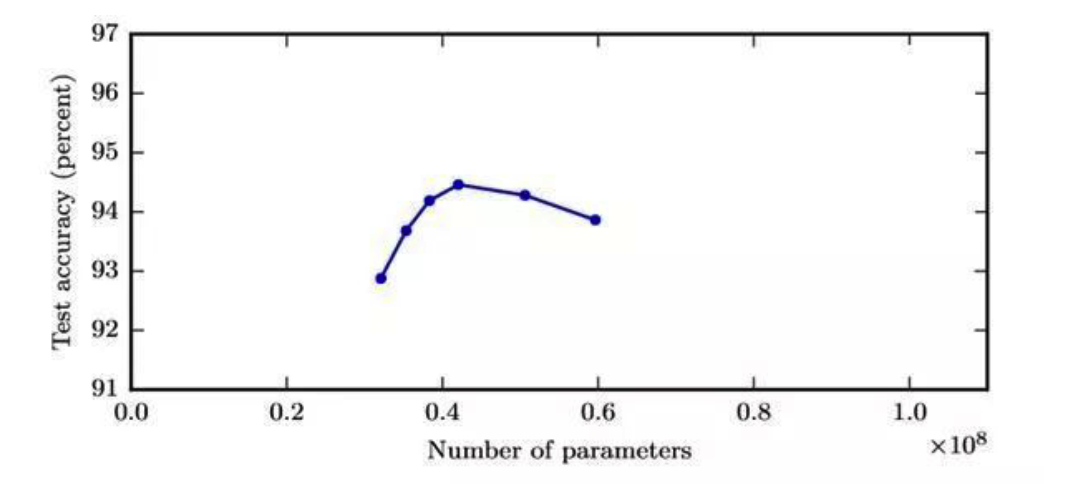
\includegraphics[width=0.6\textwidth]{./figure/fig1.png}
	\end{figure}
	从图中趋势可见,如果增加神经网络的宽度,精确度会增加到一个特定阈值后,便开始降低。造成这一现象的可能原因是什么?\paren[C]
	\begin{choices}
		\item 即使增加卷积核的数量,只有少部分的核会被用作预测
		\item 当卷积核数量增加时,神经网络的预测能力会降低
		\item 当卷积核数量增加时,导致过拟合
		\item 以上都不正确
	\end{choices}
\end{question}

\begin{question}
	假设你需要调整超参数来最小化代价函数 (cost function),会使用下列哪项技术?\paren[D]
	\begin{choices}
		\item 穷举搜索
		\item 随机搜索
		\item Bayesian 优化
		\item 都可以
	\end{choices}
\end{question}

\begin{question}
	构建一个神经网络,将前一层的输出和它自身作为输入。下列哪一种架构有反馈连接?\paren[A]
	\begin{choices}
		\item 循环神经网络
		\item 卷积神经网络
		\item 限制玻尔兹曼机
		\item 都不是
	\end{choices}
\end{question}

\begin{question}
	下列哪项关于模型能力 (model capacity) 的描述是正确的?(指神经网络模型能拟合复杂函数的能力)\paren[A]
	\begin{choices}
		\item 隐藏层层数增加,模型能力增加
		\item Dropout 的比例增加,模型能力增加
		\item 学习率增加,模型能力增加
		\item 都不正确
	\end{choices}
\end{question}

\begin{question}
	在训练神经网络时,损失函数(loss)在最初的几个 epochs 时没有下降,可能的原因是?\paren[D]
	\begin{choices}
		\item 学习率(learning rate)太低
		\item 正则参数太高
		\item 陷入局部最小值
		\item 以上都有可能
	\end{choices}
\end{question}

\begin{question}
	下列哪一项属于特征学习算法 (representation learning algorithm)?\paren[C]
	\begin{choices}
		\item K 近邻算法
		\item 随机森林
		\item 神经网络
		\item 都不属于
	\end{choices}
\end{question}

\begin{question}
	假设我们拥有一个已完成训练的、用来解决车辆检测问题的深度神经冈络模型,训练所用的数据集由汽车和卡车的照片构成,而训练目标是检测出每种车辆的名称(车辆共有10 种类型)。现在想要使用这个模型来解决另外一个问题,问题数据集中仅包含一种车(福特野马)而目标变为定位车辆在照片中的位置。\paren[B]
	\begin{choices}
		\item 除去神经网络中的最后一层,冻结所有层然后重新训练
		\item 对神经网络中的最后几层进行微调,同时将最后一层(分类层)更改为回归层
		\item 使用新的数据集重新训练模型
		\item 所有答案均不对
	\end{choices}
\end{question}

\begin{question}
	假设你有5个大小为 $7 \times 7$、边界值为 0 的卷积核,同时卷积神经网络第一层的深度为1。此时如果你向这一层传入一个维度为 $224 \times 224 \times 3$ 的数据,那么神经网络下一层所接收到的数据维度是多少?\paren[A]
	\begin{choices}
		\item $218 \times 218 \times 5$
		\item $217 \times 217 \times 8$
		\item $217 \times 217 \times 3$
		\item $220 \times 220 \times 5$
	\end{choices}
\end{question}

\begin{question}
	假设我们有一个使用 ReLU 激活函数(ReLU activation function)的神经网络,假如我们把 ReLU 激活替换为线性激活,那么这个神经网络能够模拟出同或函数(XNOR function)吗?\paren[D]
	\begin{choices}
		\item 可以
		\item 不好说
		\item 不一定
		\item 不能
	\end{choices}
\end{question}

\begin{question}
	下列的哪种方法可以用来降低深度学习模型的过拟合问题?
	
	1增加更多的数据 2使用数据扩增技术 3使用归纳性更好的架构 4正规化数据 5降低架构的复杂度\paren[D]
	\begin{choices}
		\item 1 4 5
		\item 1 2 3
		\item 1 3 4 5
		\item 都有用
	\end{choices}
\end{question}

\begin{question}
	下图是一个利用 sigmoid 函数作为激活函数的含四个隐藏层的神经网络训练的梯度下降图。这个神经网络遇到了梯度消失的问题。下面哪个叙述是正确的?\paren[A]
	\begin{figure}[htbp]
		\centering
		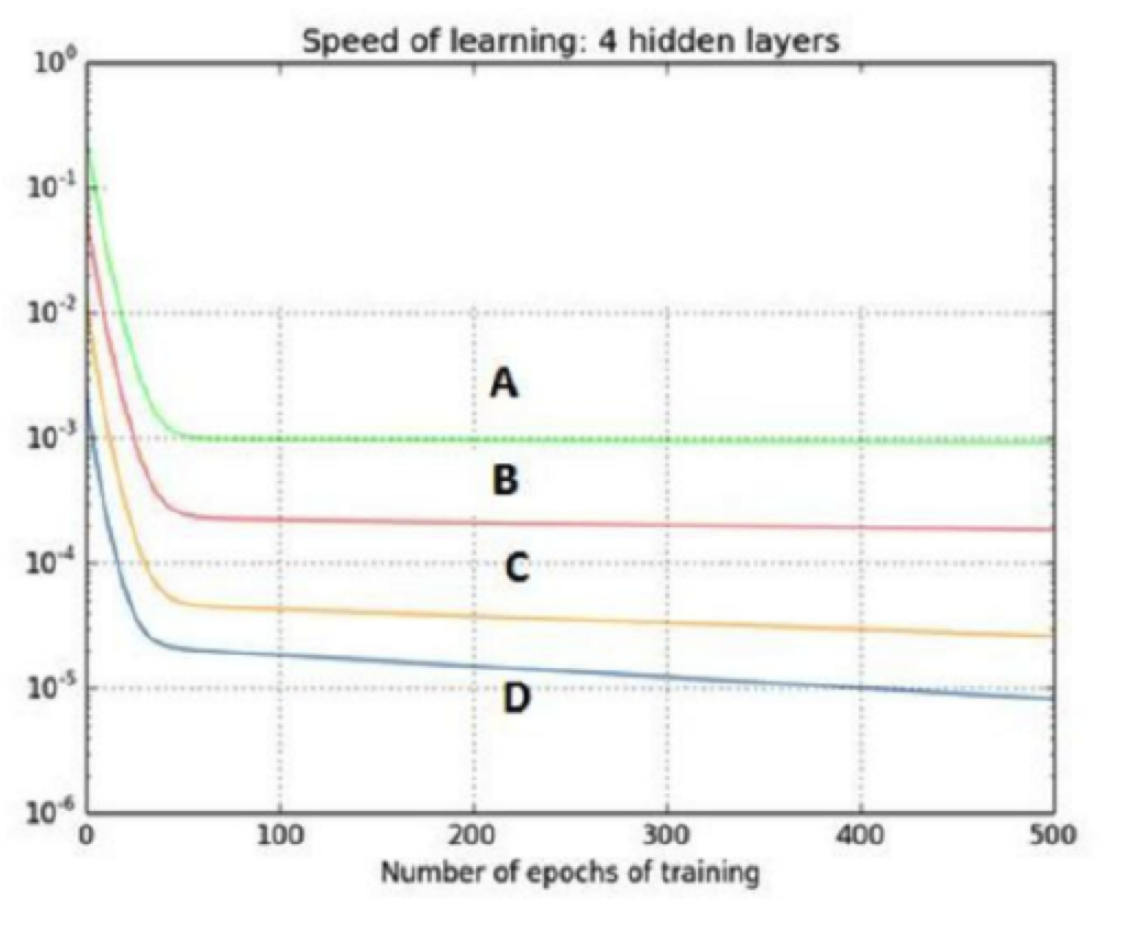
\includegraphics[width=0.4\textwidth]{./figure/fig2.png}
	\end{figure}
	\begin{choices}
		\item 第一隐藏层对应D,第二隐藏层对应C,第三隐藏层对应B,第四隐藏层对应A
		\item 第一隐藏层对应A,第二隐藏层对应C,第三隐藏层对应B,第四隐藏层对应D
		\item 第一隐藏层对应A,第二隐藏层对应B,第三隐藏层对应C,第四隐藏层对应D
		\item 第一隐藏层对应B,第二隐藏层对应D,第三隐藏层对应C,第四隐藏层对应A
	\end{choices}
\end{question}

\begin{question}
	考虑某个具体问题时,你可能只有少量数据来解决这个问题。不过幸运的是你有一个类似问题己经预先训练好的神经网络。可以用下面哪种方法来利用这个预先训练好的网络?\paren[C]
	\begin{choices}
		\item 把除了最后一层外所有的层都冻结,重新训练最后一层
		\item 对新数据重新训练整个模型
		\item 只对最后几层进行调参 (fine tune)
		\item 对每一层模型进行评估,选择其中的少数来用
	\end{choices}
\end{question}

\begin{question}
	在选择神经网络的深度时,下面哪些参数需要考虑?\begin{enumerate}
		\item 神经网络的类型(如 MLP,CNN)
		\item 输入数据
		\item 计算能力(硬件和软件能力决定)
		\item 学习速率
		\item 映射的输出函数
	\end{enumerate}\paren[C]
	\begin{choices}
		\item 1, 2, 4, 5
		\item 2, 3, 4, 5
		\item 都需要考虑
		\item 1, 3, 4, 5
	\end{choices}
	\begin{solution}
		解析:所有上述因素对于选择神经网络模型的深度都是重要的。特征抽取所需分层越多,输入数据维度越高,映射的输出函数非线性越复杂,所需深度就越深.另外为了达到最佳效果,增加深度所带来的参数量增加,也需要考虑硬件计算能力和学习速率以设计合理的训练时间。
	\end{solution}
\end{question}

\begin{question}
	当数据过大以至于无法在RAM 中同时处理时,哪种梯度下降方法更加有效?\paren[A]
	\begin{choices}
		\item 随机梯度下降法
		\item 不知道
		\item 整批梯度下降法
		\item 都不是
	\end{choices}
\end{question}

\begin{question}
	基于二次准则函数的 H-K 算法较之于感知器算法的优点是?\paren[B]
	\begin{choices}
		\item 计算量小
		\item 可以判别问题是否线性可分
		\item 其解完全适用于非线性可分的情况
	\end{choices}
	\begin{solution}
		HK 算法思想很朴实,就是在最小均方误差准则下求得权矢量。他相对于感知器算法的优点在于,他适用于线性可分和非线性可分的情况,对于线性可分的情况,给出最优权矢量,对于非线性可分得情况,能够判别出来,以退出迭代过程。
	\end{solution}
\end{question}

\begin{question}
	在一个神经网络中,知道每一个神经元的权重和偏差是最重要的一步。如果知道了神经元准确的权重和偏差,便可以近似任何函数,但怎么获知每个神经的权重和偏移呢?\paren[B]
	\begin{choices}
		\item 搜索每个可能的权重和偏差组合,直到得到最佳值
		\item 赋予一个初始值,然后检查跟最佳值的差值,不断迭代调整权重(梯度下降)
		\item 随机赋值,听天由命
		\item 以上都不正确的
	\end{choices}
\end{question}

\begin{question}
	混沌度(Perplexity)是一种常见的应用在使用深度学习处理 NLP 问题过程中的评估技术,关于混沌度, 哪种说法是正确的?\paren[B]
	\begin{choices}
		\item 混沌度没什么影响
		\item 混沌度越低越好
		\item 混沌度越高越好
		\item 混沌度对于结果的影响不一定
	\end{choices}
\end{question}

\begin{question}
	训练神经网络过程中,损失丽数在一些时期(Epoch)不再减小,原因可能是:

	1.学习率太低 2.正则参数太大 3.卡在了局部最小值\paren[D]
	\begin{choices}
		\item 1, 2
		\item 2, 3
		\item 1, 3
		\item 都是
	\end{choices}
\end{question}

\begin{question}
	我们不是想要绝对零误差,而是设置一个称为贝叶斯(bayes)误差(我们希望实现的误差)的度量。 使用贝叶斯(bayes)误差的原因是什么?\paren[D]
	\begin{choices}
		\item 输入变量可能不包含有关输出变量的完整信息
		\item 系统(创建输入-输出映射)可以是随机的
		\item 有限的训练数据
		\item 所有
	\end{choices}
\end{question}


% \section{填空题:本题共 4 小题,每小题 5 分,共 20 分。}

% % 13.
% \begin{question}
%   已知函数 $f(x) = x^3 (a \cdot 2^x - 2^{-x})$ 是偶函数,则 $a = $ \fillin[$1$] 。
% \end{question}

% % 15.
% \begin{question}
%   函数 $f(x) = |2x - 1| - 2 \ln x$ 的最小值为 \fillin[width = 4em][] 。
% \end{question}

% \begin{question}
%   某校学生在研究民间剪纸艺术时,发现剪纸时经常会沿纸的某条对称轴把纸对折。
%   规格为 \qtyproduct{20 x 12}{dm} 的长方形纸,对折 $1$ 次共可以得到
%   \qtyproduct{10 x 12}{dm}, \qtyproduct{20 x 6}{dm} 两种规格的图形,
%   它们的面积之和 $S_1 = \qty{240}{dm^2}$,
%   对折 $2$ 次共可以得到 \qtyproduct{5 x 12}{dm},\qtyproduct{10 x 6}{dm},
%   \qtyproduct{20 x 3}{dm} 三种规格的图形,它们的面积之和 $S_2 = \qty{240}{dm^2}$,
%   以此类推。则对折 $4$ 次共可以得到不同规格图形的种数为 \fillin ;
%   如果对折 $n$ 次,那么 $\sum_{k=1}^n S_k = $ \fillin \unit{dm^2}。
% \end{question}



% \section{解答题:本题共 6 小题,共 70 分。解答应写出文字说明、证明过程或者演算步骤。}

% % 17.
% \begin{problem}[points = 10]
%   已知数列 $\{a_n\}$ 满足 $a_1 = 1$,$a_{n+1} =
%     \begin{cases}
%       a_n + 1, \quad \text{$n$ 为奇数,} \\
%       a_n + 2, \quad \text{$n$ 为偶数。}
%     \end{cases}$
%   \begin{enumerate}
%     \item 记 $b_n = a_{2n}$,写出 $b_1$,$b_2$,并求数列 $\{b_n\}$ 的通项公式;
%     \item 求 $\{a_n\}$ 的前 $20$ 项和。
%   \end{enumerate}
% \end{problem}

% % 18.
% \begin{problem}[points = 12]
%   某学校组织“一带一路”知识竞赛,有 A,B 两类问题。
%   每位参加比赛的同学现在两类问题中选择一类并从中随机抽取一个问题回答,
%   若回答错误则该同学比赛结束;
%   若回答正确则从另一类问题中再随机抽取一个问题回答,无论回答正确与否,该同学比赛结束。
%   A 类问题中的每个问题回答正确的 $20$ 分,否则得 $0$ 分;
%   B 类问题中的每个问题回答正确的 $80$ 分,否则得 $0$ 分。

%   已知小明能正确回答 A 类问题的概率为 $0.8$,能正确回答 B 类问题的概率为 $0.6$,
%   且能正确回答问题的概率与回答次序无关。
%   \begin{enumerate}
%     \item 若小明先回答 A 类问题,记 $X$ 为小明的累计得分,求 $X$ 的分布列;
%     \item 为使累计得分的期望最大,小明应选择先回答哪类问题?并说明理由。
%   \end{enumerate}
% \end{problem}

% % 19.
% \begin{problem}[points = 12]
%   记 $\triangle ABC$ 的内角 $A$,$B$,$C$ 的对边分别为 $a$,$b$,$c$。
%   已知 $b^2 = ac$,点 $D$ 在边 $AC$ 上,$BD \sin\angle ABC = a \sin C$。
%   \nopagebreak
%   \begin{enumerate}
%     \item 证明:$BD = b$;
%     \item 若 $AD = 2 DC$,求 $\cos\angle ABC$。
%   \end{enumerate}
% \end{problem}

% \begin{problem}[points = 12]
%   \textfigure{
%     如图,在三棱锥 $A$-$BCD$ 中,$\text{平面} ABD \perp \text{平面} BCD$,
%     $AB = AD$,$O$ 为 $BD$ 的重点。
%     \begin{enumerate}
%       \item 证明:$OA \perp CD$;
%       \item 若 $\triangle OCD$ 是变长为 $1$ 的等边三角形,点 $E$ 在棱 $AD$ 上,
%         $DE = 2 EA$,且二面角 $E$-$BC$-$D$ 的大小为 \ang{45},
%         求三棱锥 $A$-$BCD$ 的体积。
%     \end{enumerate}
%   }{
%     \includegraphics[width=3cm]{example-image.png}
%   }
% \end{problem}

% % 21.
% \begin{problem}[points = 12]
%   在平面直角坐标系 $xOy$ 中,已知点 $F_1 (-\sqrt{17}, 0)$,$F_2 (\sqrt{17}, 0)$,
%   点 $M$ 满足 $|M F_1| - |M F_2| = 2$。记 $M$ 的轨迹为 $C$。
%   \begin{enumerate}
%     \item 求 $C$ 的方程;
%     \item 设点 $T$ 在直线 $x = \frac{1}{2}$ 上,过 $T$ 的两条直线分别交 $C$ 于 $A$,
%       $B$ 亮点和 $P$,$Q$ 亮点,且 $|TA| \cdot |TB| = |TP| \cdot |TQ|$,
%       求直线 $AB$ 的斜率与直线 $PQ$ 的斜率之和。
%   \end{enumerate}
% \end{problem}

% % 22.
% \begin{problem}[points = 12]
%   已知函数 $f(x) = x (1 - \ln x)$。
%   \begin{enumerate}
%     \item 讨论 $f(x)$ 的单调性;
%     \item 设 $a$,$b$ 为两个不相等的正数,且 $b \ln a - a \ln b = a - b$,
%       证明:$2 < \frac{1}{a} + \frac{1}{b} < \eu$。
%   \end{enumerate}
% \end{problem}

% \begin{solution}
%   函数的定义域为 $(0, +\infty)$,
%   又 \[f^{\prime}(x) = 1 - \ln x-1 = -\ln x, \score{2}\]
%   当 $x \in(0, 1)$ 时, $f^{\prime}(x) > 0$, 当 $x \in(1, +\infty)$ 时, $f^{\prime}(x) < 0$,
%   故 $f(x)$ 的递增区间为 $(0,1)$, 递减区间为 $(1, +\infty)$.
% \end{solution}


\end{document}